\chapter{Related Work}
\label{cha:related-work}

\section{LiDAR for Indoor UAV Perception}

Light Detection and Ranging (LiDAR) has become one of the most widely used sensing technologies for three-dimensional (3D) environment perception. By measuring the time-of-flight of laser pulses reflected by surrounding objects, LiDAR sensors generate point clouds containing accurate geometric information. Unlike passive vision systems, LiDAR provides direct depth measurements and operates independently of ambient illumination, making it particularly suitable for robotics, mapping, navigation, and inspection applications \cite{Guo2020DeepLearningSurvey,Li2020DeepLearningLiDARReview}.

Recent advances in sensor miniaturization have enabled the integration of lightweight LiDAR sensors into Unmanned Aerial Vehicles (UAVs) more commonly known as drones. This combination provides a flexible platform for the inspection and monitoring of indoor environments such as warehouses, industrial facilities, logistics centers, and tunnels, where human access may be difficult or hazardous \cite{Bournez2024Indoor}.

Indoor UAV perception differs significantly from conventional outdoor aerial perception. Unlike outdoor systems, indoor UAVs operate in GNSS-denied (Global Navigation Satellite System) environments and therefore rely exclusively on onboard sensors for localization and mapping. In addition, indoor scenes are characterized by cluttered geometries, severe occlusions, dynamic obstacles, and limited available datasets, which complicate both perception and navigation tasks \cite{Suleymanoglu2022IndoorMappingLiDAR,Bournez2024Indoor}.

Point clouds acquired from UAV-mounted LiDAR sensors also exhibit characteristics that distinguish them from data captured by static terrestrial scanners. Variations in sensor viewpoint, flight trajectory, object distance, and platform motion often produce irregular point densities and partial observations. Consequently, models trained on conventional indoor datasets may not generalize effectively to UAV-acquired data \cite{Armeni2016S3DIS,Bournez2024Indoor}.

Table \ref{tab:indoor_outdoor_comparison} summarizes the main differences between indoor and outdoor UAV perception scenarios.

\begin{table}[H]
\centering
\caption{Comparison between outdoor and indoor UAV LiDAR perception scenarios.}
\label{tab:indoor_outdoor_comparison}
\begin{tabular}{|l|c|c|}
\hline
\textbf{Aspect} & \textbf{Outdoor UAV} & \textbf{Indoor UAV} \\
\hline
Localization & GNSS-assisted & GNSS-denied \\
\hline
Environment scale & Large-scale & Confined spaces \\
\hline
Occlusions & Moderate & Severe \\
\hline
Point density variation & Moderate & High \\
\hline
Dataset availability & Extensive & Limited \\
\hline
Dynamic obstacles & Moderate & Frequent \\
\hline
\end{tabular}
\end{table}



%-----------------------------------------------------------
\section{Point Cloud Classification and Semantic Segmentation}
\label{sec:classification_segmentation}

The semantic interpretation of LiDAR point clouds can be formulated at different levels of granularity. The most common tasks are classification, semantic segmentation, and instance segmentation.

In point cloud classification, a single label is assigned to an entire point cloud or object. Typical examples include determining whether a segmented object corresponds to a building, a vehicle, or vegetation. While classification provides high-level scene understanding, it does not describe the spatial distribution of semantic categories within the point cloud.

Semantic segmentation extends this concept by assigning a semantic label to every point in the scene. Given a point cloud

\[
P = \{p_1,p_2,\ldots,p_n\},
\]

where each point is represented by its spatial coordinates and optional attributes such as intensity or reflectivity, the objective is to predict a semantic class

\[
y_i \in \{1,\ldots,C\}
\]

for each point \(p_i\).

This enables a detailed understanding of the environment by distinguishing between different objects and structures present in the scene \cite{Guo2020DeepLearningSurvey,Li2020DeepLearningLiDARReview}.

A more advanced task is instance segmentation, where points belonging to the same semantic category are additionally grouped into individual object instances. For example, semantic segmentation may classify multiple people as belonging to the class \textit{person}, whereas instance segmentation further separates each individual person into a distinct object instance.

Semantic segmentation has become one of the most important perception tasks in robotics and autonomous systems because it provides dense environmental information while preserving the geometric structure of the scene. In indoor UAV applications, semantic segmentation supports navigation, obstacle avoidance, mapping, and scene understanding. In particular, the reliable identification of human operators is essential for ensuring safe interaction between UAVs and people in industrial and logistics environments.

Recent advances in deep learning have significantly improved semantic segmentation performance by enabling the direct extraction of geometric features from raw point clouds. As a result, modern architectures have largely replaced traditional approaches based on handcrafted descriptors and conventional machine learning techniques \cite{Qi2017PointNet,Qi2017PointNetPP}.


\section{Deep Learning Architectures for Point Cloud Segmentation}
\label{sec:dl_architectures}

The development of deep learning methods has fundamentally transformed point cloud semantic segmentation. Early approaches relied on handcrafted geometric descriptors, such as surface normals, curvature, roughness, and height features, combined with traditional machine learning classifiers including Support Vector Machines (SVMs) and Random Forests. Although these methods were computationally efficient, their performance strongly depended on manual feature engineering and often lacked robustness when applied to different environments \cite{Guo2020DeepLearningSurvey,Li2020DeepLearningLiDARReview,Zhao2021TechnicalSurveyPointCloudClustering}.

Modern deep learning architectures learn discriminative geometric representations directly from raw point clouds, eliminating the need for handcrafted features. Existing methods can be broadly categorized into point-based, convolution-based, and transformer-based networks. Among these, point-based methods have been particularly influential due to their ability to process unordered point sets directly while preserving the original geometric information.

\subsection{Point-Based Networks}

PointNet \cite{Qi2017PointNet} was the first neural network capable of directly processing unordered point clouds. Its key contribution is the use of shared multilayer perceptrons (MLPs) combined with a symmetric pooling function, ensuring permutation invariance while learning point-wise features. Despite its simplicity and efficiency, PointNet processes each point independently before global aggregation, limiting its ability to capture local geometric structures that are essential for semantic segmentation.

To overcome this limitation, PointNet++ \cite{Qi2017PointNetPP} introduced a hierarchical feature learning strategy inspired by convolutional neural networks. The architecture recursively samples points, groups local neighborhoods, and applies PointNet operations at multiple scales. This hierarchical aggregation enables the network to capture both fine local geometry and global contextual information, making PointNet++ one of the most influential baseline architectures for point cloud segmentation.

Dynamic Graph CNN (DGCNN) \cite{Wang2019DGCNN} further improved local feature learning by dynamically constructing a graph in the feature space at every network layer. Instead of relying on fixed spatial neighborhoods, DGCNN updates the graph according to the learned feature embeddings and employs the EdgeConv operator to model relationships between neighboring points. This dynamic representation significantly enhances the extraction of local geometric patterns and object boundaries, achieving competitive performance across numerous segmentation benchmarks.

More recently, PointVector \cite{PointVector} introduced vector-based feature aggregation to improve geometric representation learning. Rather than treating features as independent scalar channels, PointVector explicitly models both magnitude and directional information within local neighborhoods. This richer geometric encoding enables more expressive feature interactions while maintaining computational efficiency, leading to improved segmentation performance on challenging indoor and outdoor datasets.

PointNeXt \cite{PointNeXt} revisits the PointNet++ architecture from a modern perspective. Instead of proposing a completely new operator, PointNeXt demonstrates that substantial performance gains can be achieved through improved training strategies, architectural refinements, residual connections, optimized normalization, and better scaling. These modifications significantly narrow the performance gap with more complex architectures while preserving the simplicity and efficiency of the PointNet++ design.

Overall, the evolution from PointNet to PointNet++, DGCNN, PointVector, and PointNeXt illustrates the progressive enhancement of local feature extraction and geometric representation learning, establishing these architectures as fundamental references for point cloud semantic segmentation.

\subsection{Other Deep Learning Architectures}

Beyond point-based networks, several alternative architectures have demonstrated excellent performance for semantic segmentation.

Convolution-based methods, such as KPConv \cite{Thomas2019KPConv}, adapt convolution operations to irregular point clouds through kernel point convolutions, providing highly accurate local feature extraction. RandLA-Net \cite{Hu2020RandLANet} focuses on efficient large-scale processing by combining random sampling with lightweight local feature aggregation, making it particularly suitable for real-time applications.

Transformer-based architectures, represented by Point Transformer \cite{Zhao2021PointTransformer}, leverage self-attention mechanisms to capture long-range contextual dependencies between points. Subsequent transformer variants have achieved state-of-the-art segmentation accuracy on several benchmarks \cite{PTMF2025,Robert20233DLST}, although these improvements generally come at the cost of higher computational and memory requirements.

Although transformer-based architectures currently achieve state-of-the-art performance on several semantic segmentation benchmarks, their high computational complexity, memory consumption, and inference latency make them less suitable for deployment on resource-constrained edge devices, such as embedded computers onboard UAVs. Similarly, convolution-based methods such as KPConv provide excellent segmentation accuracy but rely on computationally expensive neighborhood convolution operations that increase execution time and memory usage. Since the objective of this work is to investigate semantic segmentation for online edge computing scenarios, point-based architectures offer a more favorable trade-off between computational efficiency, scalability, and segmentation performance. Consequently, this work focuses on PointNet++, DGCNN, PointVector, and PointNeXt, which provide competitive accuracy while maintaining lower computational requirements and are therefore better suited for real-time UAV applications.

\subsection{Comparison of Representative Architectures}

Table \ref{tab:architecture_comparison} summarizes the main characteristics of representative architectures commonly employed for point cloud semantic segmentation.

\begin{table}[H]
\centering
\caption{Comparison of representative point cloud segmentation architectures.}
\label{tab:architecture_comparison}
\begin{tabular}{|l|p{3.2cm}|p{3.3cm}|p{3.2cm}|}
\hline
\textbf{Architecture} & \textbf{Main Idea} & \textbf{Advantages} & \textbf{Limitations} \\
\hline
PointNet \cite{Qi2017PointNet} & Independent point feature learning with symmetric pooling & Simple, efficient, permutation invariant & Limited local context modeling \\
\hline
PointNet++ \cite{Qi2017PointNetPP} & Hierarchical neighborhood aggregation & Strong local and global feature extraction & Higher computational cost \\
\hline
DGCNN \cite{Wang2019DGCNN} & Dynamic graph learning with EdgeConv & Excellent local geometry modeling & Dynamic graph construction increases complexity \\
\hline
PointVector \cite{PointVector} & Vector-based local feature aggregation & Rich geometric representation & Higher computational overhead than PointNet++ \\
\hline
PointNeXt \cite{PointNeXt} & Modernized PointNet++ architecture & Improved accuracy with efficient design & Still limited compared to transformer global modeling \\
\hline
KPConv \cite{Thomas2019KPConv} & Kernel point convolutions & High segmentation accuracy & Computationally demanding \\
\hline
RandLA-Net \cite{Hu2020RandLANet} & Random sampling with local aggregation & Efficient large-scale processing & Limited global context \\
\hline
Point Transformer \cite{Zhao2021PointTransformer} & Self-attention mechanisms & Strong contextual reasoning & High memory and computational cost \\
\hline
\end{tabular}
\end{table}

Among the existing approaches, PointNet++, DGCNN, PointVector, and PointNeXt represent the main evolutionary line of point-based architectures, progressively improving local geometric representation while maintaining direct processing of raw point clouds. Convolution-based methods such as KPConv and efficient architectures like RandLA-Net remain strong alternatives, whereas transformer-based models provide the highest representational capacity at the expense of greater computational complexity. These architectures constitute the primary candidates for transfer learning and adaptation to UAV LiDAR semantic segmentation tasks.\cite{pang2022pointmae}
\section{Human Detection in LiDAR Point Clouds}
\label{sec:human_detection}

Human detection is a fundamental perception task in autonomous systems operating in shared environments. In the context of indoor UAV applications, the reliable identification of people is particularly important for collision avoidance, human-aware navigation, industrial safety monitoring, and inspection tasks. Consequently, detecting and segmenting human operators within LiDAR point clouds has attracted increasing attention in recent years.

Early approaches to human detection relied on handcrafted geometric descriptors combined with conventional machine learning algorithms. Typical pipelines included point cloud clustering, feature extraction, and object classification. Techniques such as Euclidean clustering, density-based clustering, and shape analysis were commonly used to isolate candidate objects before applying classifiers such as Support Vector Machines (SVMs) or Random Forests. Although these methods achieved reasonable performance in controlled environments, they often struggled with partial occlusions, varying viewpoints, and complex indoor scenes.

The emergence of deep learning significantly improved human detection capabilities by enabling the automatic extraction of discriminative geometric features directly from raw point cloud data. Architectures originally developed for  multiclass semantic segmentation, including the previously mentioned, have demonstrated the ability to distinguish human structures from surrounding objects and background elements.\cite{Lorente2021PedestrianPointNet}

Unlike object classification, semantic segmentation provides point-level predictions, allowing the precise localization of human subjects within the environment. This capability is particularly valuable for UAV applications, where accurate spatial information is required to support navigation and safety-critical decision making.

Despite recent advances, human detection in indoor LiDAR data remains challenging. Human bodies often appear only partially visible due to occlusions caused by furniture, machinery, shelves, or other environmental structures. Furthermore, variations in posture, clothing, movement, and sensor viewpoint can significantly alter the geometric appearance of a person within the point cloud.\cite{Ferreira2023PedestrianLiDAR}  These challenges become even more pronounced in UAV-acquired datasets, where changes in altitude and viewing angle introduce additional variability.

Another important limitation is the scarcity of publicly available datasets specifically designed for indoor UAV-based human detection. Most existing benchmarks focus either on static terrestrial scanning or on general semantic segmentation tasks, where the \textit{person} class is often underrepresented. As a result, the ability of pretrained models to generalize to newly acquired indoor UAV data remains insufficiently explored.

These limitations motivate the use of transfer learning techniques, where models pretrained on large semantic segmentation datasets are adapted to new environments through fine-tuning. Such approaches enable the exploitation of previously learned geometric representations while reducing the amount of annotated data required for training. Consequently, transfer learning has become a promising strategy for developing robust human detection systems in indoor UAV perception scenarios.

\section{Transfer Learning and Domain Adaptation}
\label{sec:transfer_learning}

Deep learning models for point cloud segmentation typically require large amounts of annotated data for effective training. However, the acquisition and manual annotation of LiDAR point clouds are expensive and time-consuming processes, particularly in indoor environments where point-level semantic labeling must often be performed manually. As a result, training segmentation models from scratch is frequently impractical when only a limited dataset is available.

Transfer learning has emerged as an effective strategy for addressing this limitation. The central idea is to leverage knowledge acquired from large annotated datasets and adapt pretrained models to new tasks or environments through fine-tuning. By initializing a network with pretrained weights, the model can reuse previously learned geometric representations, reducing both training time and data requirements while often improving generalization performance.\cite{pan2010survey,pang2022pointmae}

In the context of LiDAR perception, many state-of-the-art architectures are commonly pretrained on large benchmark datasets such as SemanticKITTI \cite{Behley2019SemanticKITTI}, S3DIS \cite{Armeni2016S3DIS}, or DALES \cite{Varney2020DALES}. These datasets enable models to learn generic geometric features that can subsequently be transferred to related applications.

Despite the benefits of transfer learning, significant performance degradation may occur when a model is applied to data acquired under conditions different from those encountered during pretraining. This phenomenon is commonly referred to as domain shift.\cite{jaritz2020xmuda} In LiDAR-based perception, domain shift can arise from differences in sensor characteristics, point density, acquisition viewpoints, environmental structure, or semantic class distributions.

For indoor UAV applications, domain shift represents a particularly important challenge. Most publicly available datasets have been acquired using terrestrial scanners, mobile mapping systems, or outdoor platforms, whereas UAV-mounted LiDAR sensors capture data from dynamic aerial viewpoints and under different operational conditions. Consequently, models trained on existing datasets may not generalize effectively to newly acquired indoor UAV point clouds without additional adaptation.

To mitigate this issue, fine-tuning strategies are commonly employed. During fine-tuning, a pretrained network is further trained using a smaller task-specific dataset, allowing the model to adapt its learned representations to the characteristics of the target domain. This approach has proven effective across numerous computer vision and point cloud perception tasks, especially when annotated data are limited.

Given the scarcity of indoor UAV LiDAR datasets and the high cost of point-wise annotation, transfer learning and fine-tuning provide a practical framework for developing semantic segmentation models capable of operating in new environments while minimizing the amount of required training data. Consequently, these techniques are particularly relevant for evaluating the adaptation of existing segmentation architectures to indoor UAV-based human detection scenarios.

\section{Datasets and Evaluation Metrics}
\label{sec:datasets_metrics}

\subsection{Existing Indoor LiDAR Datasets}

The development of deep learning methods for point cloud understanding has been strongly supported by the availability of publicly annotated datasets. These benchmarks provide standardized evaluation protocols and enable the comparison of semantic segmentation architectures under common conditions.

Among indoor benchmarks, the Stanford Large-Scale 3D Indoor Spaces (S3DIS) dataset \cite{Armeni2016S3DIS} remains one of the most widely adopted datasets for semantic segmentation research. S3DIS contains point clouds acquired from office buildings and educational facilities, with point-wise annotations for multiple semantic categories including walls, floors, ceilings, furniture, and structural elements. Due to its size and annotation quality, S3DIS has become a standard benchmark for evaluating indoor point cloud segmentation methods.

Another widely used benchmark is ScanNet \cite{Dai2017ScanNet}, which contains large-scale RGB-D reconstructions of indoor environments together with dense semantic annotations. ScanNet has contributed significantly to the development of indoor scene understanding algorithms and is frequently used for training and evaluating deep learning architectures.
\begin{figure}[H]
\centering
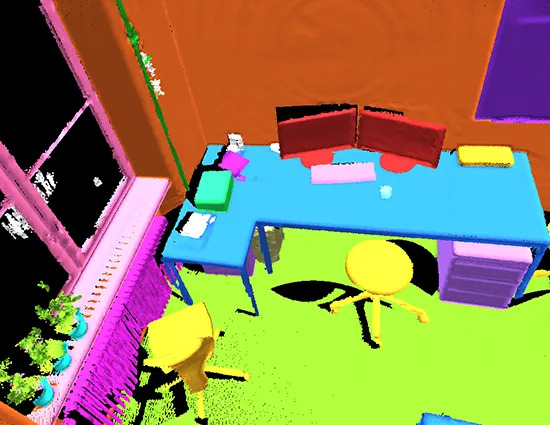
\includegraphics[width=0.55\linewidth]{S3DES.jpg}
\caption{Example of a semantically annotated scene from the S3DIS dataset \cite{Armeni2016S3DIS}.}
\label{fig:s3dis}
\end{figure}
More recently, the 3DSES dataset \cite{Merizette2025ThreeDSES} was introduced to support semantic segmentation research in industrial indoor environments. Compared with traditional office-oriented datasets, 3DSES includes scenes that better represent industrial facilities and inspection scenarios, making it particularly relevant for robotics applications.

Although this work focuses on indoor environments, aerial datasets have also played an important role in the development of LiDAR segmentation methods. For example, the DALES dataset \cite{Varney2020DALES} contains large-scale UAV-acquired point clouds with dense semantic annotations and has become a common benchmark for aerial semantic segmentation.

\begin{table}[htbp]
\centering
\caption{Representative datasets for point cloud semantic segmentation.}
\label{tab:datasets}
\begin{tabular}{|l|l|l|}
\hline
\textbf{Dataset} & \textbf{Environment} & \textbf{Acquisition Platform} \\
\hline
S3DIS \cite{Armeni2016S3DIS} & Offices and buildings & Terrestrial scanner \\
\hline
ScanNet \cite{Dai2017ScanNet} & Indoor scenes & RGB-D reconstruction \\
\hline
3DSES \cite{Merizette2025ThreeDSES} & Industrial facilities & Terrestrial scanner \\
\hline
DALES \cite{Varney2020DALES} & Outdoor aerial environments & UAV LiDAR \\
\hline
\end{tabular}
\end{table}

\subsection{Limitations of Current Datasets}

Despite the availability of several public benchmarks, existing datasets present important limitations when considering indoor UAV perception. Most indoor datasets, including S3DIS and 3DSES, were acquired using static terrestrial scanners. Consequently, they do not capture many of the characteristics associated with UAV-based data acquisition, including aerial viewpoints, platform motion, dynamic trajectories, and viewpoint-dependent density variations \cite{Armeni2016S3DIS,Bournez2024Indoor}.

Furthermore, the majority of existing datasets were designed for general semantic segmentation rather than human-centered perception tasks. As a result, the \textit{person} class is often underrepresented, limiting the evaluation of human detection and segmentation performance in realistic indoor UAV scenarios.

Another important limitation is the scarcity of publicly available datasets specifically acquired using UAV-mounted LiDAR sensors in indoor environments. This lack of representative data hinders the development and evaluation of perception systems intended for autonomous indoor flight.

These limitations motivate the creation of dedicated datasets that better reflect the operational conditions encountered by UAV-mounted LiDAR systems, particularly in applications involving human detection and navigation in GNSS-denied environments.

\subsection{Evaluation Metrics}

The performance of semantic segmentation models is commonly assessed using quantitative metrics that compare predicted labels with ground-truth annotations. Among these metrics, Overall Accuracy (OA), Intersection over Union (IoU), and mean Intersection over Union (mIoU) are the most widely reported in the literature.

Overall Accuracy measures the proportion of correctly classified points over the total number of points in the dataset. Although intuitive and easy to interpret, this metric can be misleading when class distributions are highly imbalanced.

Intersection over Union evaluates the overlap between predicted and ground-truth labels for a particular semantic class:

\[
IoU = \frac{TP}{TP + FP + FN}
\]

where \(TP\), \(FP\), and \(FN\) represent true positives, false positives, and false negatives, respectively.

The mean Intersection over Union (mIoU) is obtained by averaging the IoU values across all semantic classes. This metric is generally considered the most representative measure of segmentation performance because it mitigates the influence of class imbalance and provides a balanced evaluation across categories \cite{Behley2019SemanticKITTI,Varney2020DALES}.

Additional metrics such as Precision, Recall, and F1-score are frequently used when evaluating the performance of specific classes. These metrics are particularly relevant for human detection applications, where correctly identifying human operators is often more important than maximizing overall classification accuracy.

Among the available metrics, mIoU remains the most widely adopted benchmark for comparing semantic segmentation methods and will therefore be used as one of the primary evaluation criteria throughout this work.

\section{Research Gap and Motivation}
\label{sec:research_gap}

The literature review highlights the remarkable progress achieved in LiDAR semantic segmentation through the development of deep learning architectures such as PointNet++, KPConv, RandLA-Net, and Point Transformer. These methods have demonstrated strong performance on several benchmark datasets and have become the foundation of modern point cloud perception systems.

However, several limitations remain when considering indoor UAV applications, particularly for human detection and semantic segmentation. Based on the reviewed literature, the following research gaps can be identified:

\begin{enumerate}

\item \textbf{Limited availability of indoor UAV LiDAR datasets.}

Most publicly available datasets, including S3DIS \cite{Armeni2016S3DIS} and 3DSES \cite{Merizette2025ThreeDSES}, were acquired using terrestrial scanning systems. Consequently, they do not fully represent the characteristics of UAV-based data acquisition, such as aerial viewpoints, platform motion, and varying point densities. The lack of representative datasets limits the development and evaluation of perception systems specifically designed for indoor UAV operation.

\item \textbf{Insufficient evaluation of pretrained segmentation models on indoor UAV data.}

State-of-the-art architectures are commonly trained and evaluated on standard benchmarks. However, their ability to generalize to newly acquired indoor UAV point clouds remains insufficiently studied. Differences between source and target datasets often introduce domain shift, leading to performance degradation and motivating the need for transfer learning and fine-tuning strategies.

\item \textbf{Limited research on human detection in indoor UAV LiDAR scenarios.}

While semantic segmentation has been extensively studied, relatively few works focus specifically on the detection and segmentation of people in indoor UAV environments. Human subjects frequently appear under challenging conditions, including partial occlusions, viewpoint variations, and cluttered surroundings, making reliable detection a difficult task.

\item \textbf{Lack of comparative studies on model adaptation through fine-tuning.}

Although pretrained models are widely available, there is limited evidence regarding which architectures are better suited for adaptation to small, task-specific indoor UAV datasets. Understanding the effectiveness of different fine-tuning approaches remains an open research question.

\end{enumerate}

These research gaps directly motivate the objectives of this work. First, an indoor UAV LiDAR dataset is created to provide representative data for human detection and semantic segmentation tasks. Second, several pretrained deep learning architectures are adapted through transfer learning and fine-tuning. Finally, their performance is evaluated and compared to assess their suitability for indoor UAV perception and person segmentation applications.

\begin{table}[H]
\centering
\caption{Identified research gaps and corresponding objectives of this work.}
\label{tab:research_gap}
\begin{tabular}{|p{6cm}|p{7cm}|}
\hline
\textbf{Research Gap} & \textbf{Objective of this Work} \\
\hline
Limited availability of indoor UAV LiDAR datasets &
Create a representative indoor UAV LiDAR dataset. \\
\hline
Limited knowledge about model adaptation to UAV-acquired data &
Evaluate transfer learning and fine-tuning strategies. \\
\hline
Insufficient evaluation of human detection in indoor UAV environments &
Assess segmentation performance for the \textit{person} class. \\
\hline
Domain shift between public benchmarks and real UAV acquisitions &
Analyze the generalization capability of pretrained models. \\
\hline
\end{tabular}
\end{table}
